\begin{figure*}[t]
  \centering
  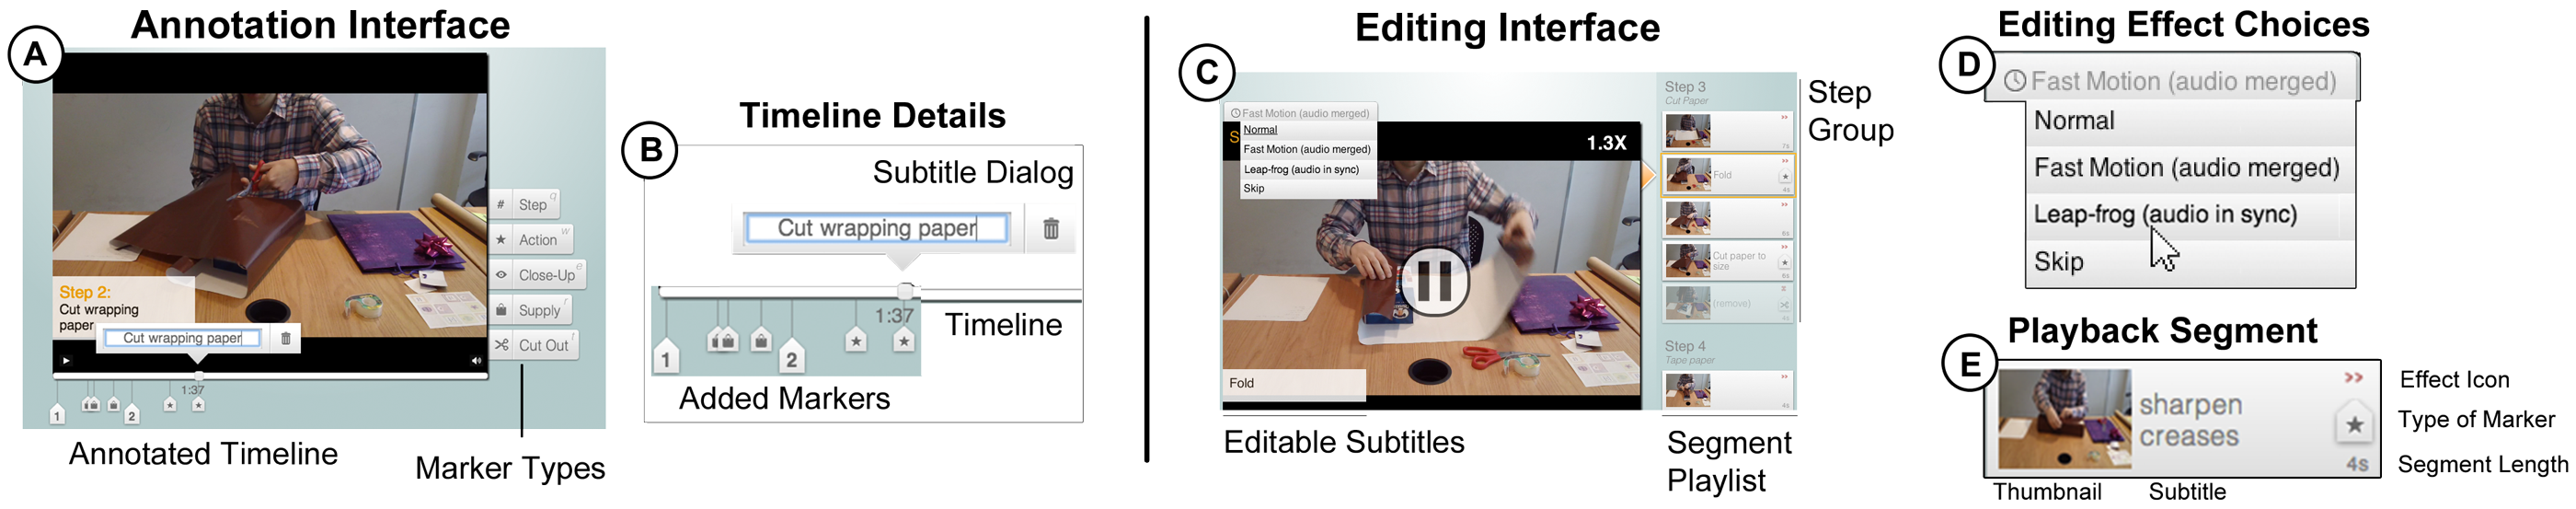
\includegraphics[width=7.0in]{\democut/fig/two-column-ui-small}
  \caption{Users first add markers to their recorded video in the Annotation Interface (A). Each marker can be labeled with a descriptive string (B). The Editing Interface shows automatically generated segments with effect suggestions (C). Users can change the effect (D) applied to each segment (E).}
  \label{fig:ui}
    \vspace{-0.15in}
\end{figure*}


\subsection{Design Implications}

Based on our analysis of existing video tutorials and interviews with
tutorial authors, we identified a few key aspects of the tutorial creation
process that have important design implications for DIY video
editing systems.

\subsubsection{Working with single take, single camera footage.}
%
Most amateur authors record demonstrations in a single take with a
a single camera. As a result, the captured footage often includes
mistakes and long, repetitive actions.

\subsubsection{Making concise videos.}
%
The most important design principle for creating effective DIY videos
is to make them concise without sacrificing clarity. To this end,
authors remove/condense unnecessary or repetitive actions so that the
resulting video only contains salient footage.

\subsubsection{Retiming audio and video tracks separately.}
%
One common technique for speeding up a video involves breaking the
synchronization between the audio and video tracks so that they can be retimed
separately. In cases where the narration refers to
specific visual events, the tracks should remain aligned.

\subsubsection{Emphasizing important information.}
%
Most effective DIY videos include titles, annotations and/or closeup
views to emphasize relevant information and highlight key details.

\subsubsection{Focusing on high-level editing decisions.}
% Editing captured footage is a difficult and time-consuming task.
Amateur users often struggle with low-level manipulation of cut points and timing in general-purpose video editors: A system should reduce the editing efforts and enable authors to focus on making simple choices for the final production.
% \bh{This point seems different from the others. It's a general complaint instead of an observation of what our participants do.}

We next describe how these considerations informed the design of DemoCut.
